\chapter{Metodologia}

        Jogos \textit{multiplayer} abrangem um espectro vasto de gêneros, incluindo MOBA (\textit{Multiplayer Online Battle Arena}), FPS (\textit{First-Person Shooter}), jogos esportivos e MMORPG (\textit{ Massively Multiplayer Online Role-Playing Game}). Cada um com dinâmicas sociais e mecânicas próprias.
        Diante dessa diversidade, e considerando que o objetivo do presente estudo é avaliar o potencial de interação social promovido pelos jogos, torna-se imprescindível reduzir ao máximo o número de variáveis envolvidas. Diversos fatores podem interferir nos resultados, como o número de jogadores simultâneos, a presença ou ausência de comunicação por voz durante as partidas, a toxicidade entre jogadores, a complexidade das mecânicas de jogo, o tempo de duração das partidas e até a natureza online ou local da interação.

        \section{Among’Us}

            \textbf{Among’Us}\footnote{https://play.google.com/store/apps/details?id=com.innersloth.spacemafia\&hl=en-US} é um jogo eletrônico \textit{multiplayer}, lançado em 2018 pela desenvolvedora InnerSloth, que combina elementos de cooperação e enganação em partidas rápidas. Ambientado em uma nave espacial (ou cenários similares), o jogo coloca de 4 a 15 jogadores em papéis divididos entre \textbf{Tripulantes} e \textbf{Impostores}.

            \begin{figure}[h]
                \centering
                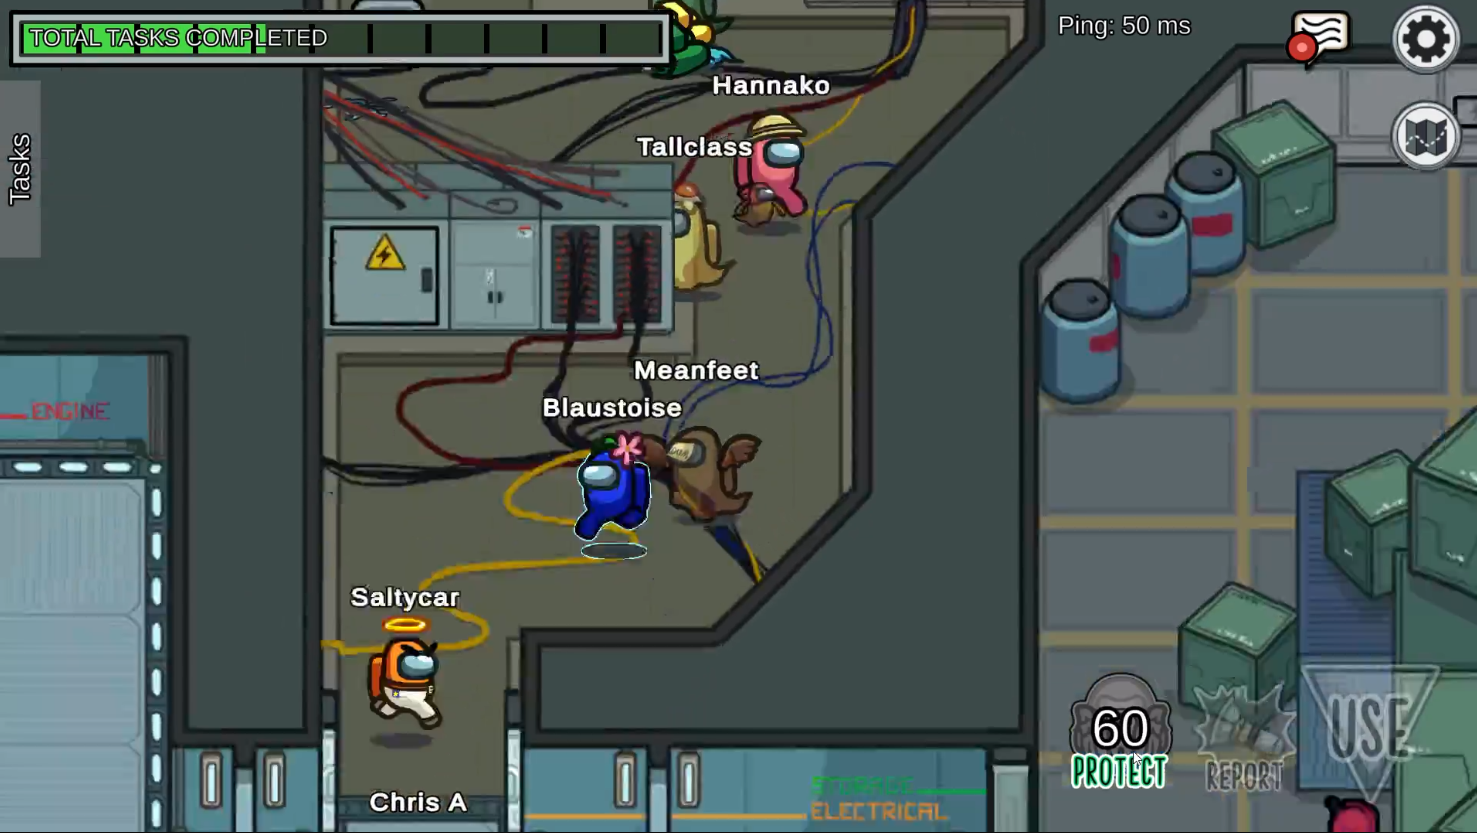
\includegraphics[width=1\textwidth]{imgs/Amongus1.png}
                \caption{Among'Us: Tela de jogo de um Tripulante}
                \label{fig:Amongus1}
                \vspace{2mm}
                \footnotesize Fonte: Próprio autor.
            \end{figure}

            O objetivo dos Tripulantes é realizar tarefas simples distribuídas pelo mapa, enquanto tentam identificar quem entre eles é o Impostor. Já os Impostores devem sabotar a missão e eliminar os tripulantes sem serem descobertos. A dinâmica principal do jogo gira em torno de reuniões nas quais os jogadores discutem, por voz ou texto, e votam em quem acham que é o impostor. Caso o resultado seja de o número de impostores ser igual ao número de tripulantes, os impostores vencem; já no caso dos tripulantes expulsarem todos os impostores ou concluírem todas as tarefas solicitadas, os tripulantes vencem.

            \begin{figure}[h]
                \centering
                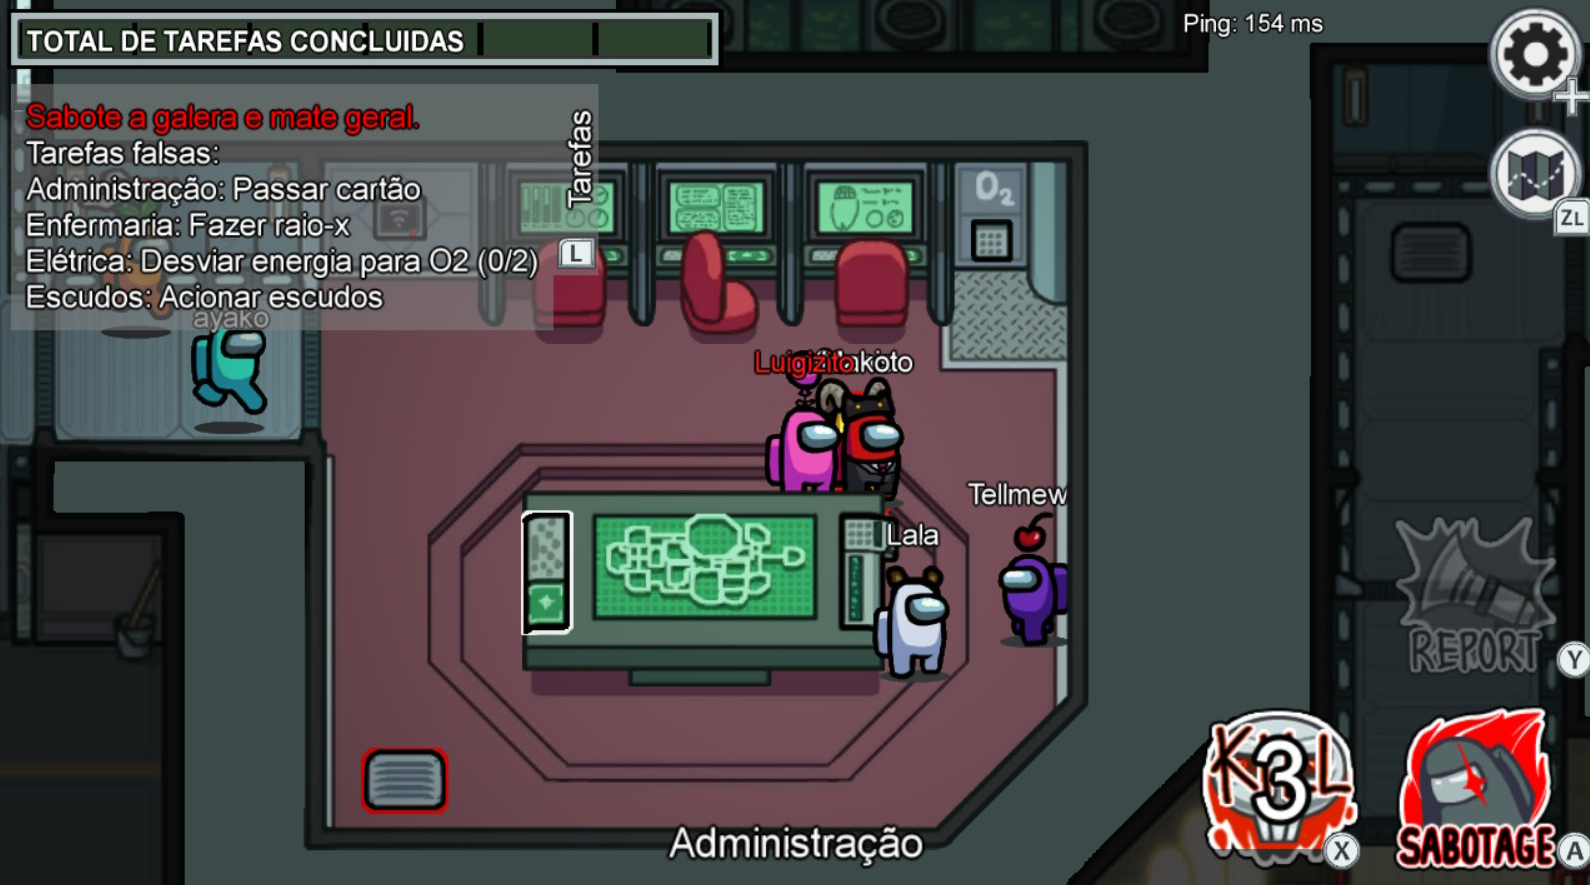
\includegraphics[width=1\textwidth]{imgs/Amongus2.png}
                \caption{Among'Us: Tela de jogo de um Impostor}
                \label{fig:Amongus2}
                \vspace{2mm}
                \footnotesize Fonte: Próprio autor.
            \end{figure}

            Em geral, o jogo força a cooperação dos indivíduos, já que a expulsão da nave é feita de forma democrática, em que o voto de todos tem o mesmo peso. Ao mesmo tempo, incentiva os impostores a criarem estratégias para não serem pegos.

    \section{Ferramentas de Avaliação de Habilidades Sociais}

        Para a avaliação das habilidades sociais dos participantes, foram  analisados alguns instrumentos reconhecidos na literatura:

        \begin{itemize}
            \item SSRS (\textit{Social Skills Rating System})\cite{Bul2016};
            \item TEIQue-SF (\textit{Trait and Emotional Intelligence Questionnaire Short Form})\cite{petrides2009teique};
            \item IHS (Inventário de Habilidades Sociais)\cite{de2006inventario}.
        \end{itemize}

        \subsection{Social Skills Rating System}

            O \textit{Social Skills Rating System (SSRS)} foi desenvolvido por \cite{GreshamElliott1990} com o objetivo de avaliar habilidades sociais e comportamentos em crianças e adolescentes. O instrumento surgiu em 1990 para suprir a necessidade de medir competências sociais de forma padronizada, oferecendo informações úteis tanto para pesquisas quanto para intervenções educacionais e clínicas.

            O SSRS é direcionado principalmente a crianças e adolescentes, podendo ser respondido por professores, pais ou pelo próprio indivíduo. Algumas adaptações permitem seu uso em adultos, especialmente em contextos educacionais ou de treinamento social.

            O instrumento mede \textbf{habilidades sociais}, como cooperação, assertividade, responsabilidade e autocontrole, bem como, agressividade, hiperatividade, ansiedade e depressão. Além disso, avalia a percepção social do indivíduo, ou seja, como ele interage com colegas, professores e familiares.

            A aplicação é realizada por meio de questionários em escala Likert, que permitem quantificar a frequência de determinados comportamentos.

        \subsection{Trait Emotional Intelligence Questionnaire – Short Form (TEIQue-SF)}

            O \textit{Trait Emotional Intelligence Questionnaire – Short Form (TEIQue-SF)} é uma versão abreviada do \textbf{TEIQue}, desenvolvido por \cite{Petrides2009}. O instrumento foi criado para medir o \textbf{traço de inteligência emocional} em indivíduos de forma prática e confiável, permitindo avaliações rápidas sem comprometer a validade do construto.

            O TEIQue-SF é direcionado a adolescentes e adultos, sendo aplicado em contextos educacionais, clínicos e de pesquisa. Ele visa avaliar a capacidade do indivíduo de perceber, compreender, expressar e regular emoções, bem como a habilidade de utilizar essas informações para guiar pensamentos e comportamentos. O instrumento é composto por 30 itens em uma escala Likert de 7 pontos (de ``discordo fortemente'' a ``concordo fortemente'').

        \subsection{Inventário de Habilidades Sociais (IHS)}

            O \textit{Inventário de Habilidades Sociais} (IHS) foi desenvolvido por \cite{DelPretteDelPrette2002} com o objetivo de avaliar de forma sistemática as habilidades sociais em contextos educativos e clínicos. O instrumento surgiu para fornecer um método padronizado de avaliação de competências sociais no Brasil.

            O IHS é direcionado a diferentes públicos, dependendo da versão utilizada. Ele permite que os avaliadores compreendam o repertório social do indivíduo e como ele se comporta em diferentes situações interpessoais, como relacionamentos familiares, escolares e profissionais.

            O instrumento investiga diferentes dimensões das habilidades sociais, organizando seus resultados em cinco fatores:
            \begin{itemize}
                \item F1 - Enfrentamento e autoafirmação com risco: relacionado à capacidade de defender direitos e expressar opiniões em situações que envolvem possíveis reações negativas;
                \item F2 - Autoafirmação na expressão de sentimento positivo: que avalia a capacidade de expressar sentimentos positivos e afetividade;
                \item F3 - Conversação e desenvoltura social: associado à capacidade de iniciar, manter e encerrar conversas e interações sociais;
                \item F4 - Autoexposição a desconhecidos e situações novas: que investiga a desenvoltura em interações com pessoas desconhecidas e em situações pouco familiares;
                \item F5 - Autocontrole da agressividade: relacionado à capacidade de controlar reações agressivas diante de situações interpessoais adversas.
            \end{itemize}

        A avaliação é realizada por meio de um questionário de autorrelato, utilizando uma escala de frequência dos comportamentos apresentados em diferentes situações sociais. As respostas permitem a obtenção de escores quantitativos, possibilitando a análise do repertório geral de habilidades sociais e de suas diferentes dimensões.

        Devido a ser a ferramenta que melhor se enquadra a proposta desta pesquisa, o \textbf{IHS} foi escolhido para analisar os dados dos voluntários. Isto também se deve a algumas características específicas da população de voluntários. É importante salientar que a aplicação desta ferramenta não requer formação específica, mas a interpretação adequada dos resultados exige conhecimento técnico de psicologia ou áreas afins, para garantir que as informações obtidas foram interpretadas da forma correta foi convidado um profissional qualificado.

    \section{Coleta e escolha dos voluntários}
    A coleta dos voluntários foi realizada por meio de um questionário online divulgado de duas principais formas: em fóruns e servidores relacionados a comunidades de jogos \textit{multiplayer} — em especial servidores da plataforma \textbf{Discord}\footnote{https://discord.com} — e em redes sociais, e em posters colados por toda a região da Universidade Federal do Rio Grande. O questionário de triagem reuniu dados demográficos (idade, sexo, escolaridade); todas as perguntas do \textbf{IHS} para uma primeira análise; informações sobre o hábito de jogo (frequência, títulos mais jogados, experiência com jogos \textit{multiplayer}); e a autodeclaração de diagnóstico de TDAH (quando aplicável) \footnote{Esta informação não avaliada no presente trabalho, mas presente para possíveis estudos futuros}.


    Como forma de incentivo à participação, os voluntários que completassem todas as etapas do experimento foram incluídos em um sorteio de vale-presentes, semelhante a abordagens utilizadas nos trabalhos de \cite{Maloney2020, Brakel2023}, conforme detalhado no termo de consentimento informado\footnote{Essa prática tem sido reconhecida na literatura como uma forma eficaz e eticamente aceitável de reforçar a participação em pesquisas com intervenção mínima, desde que os sorteios sejam devidamente informados no termo de consentimento e não configurem forma de coerção.}. No entanto, mesmo com o incentivo a coleta dos voluntários foi um dos maiores desafios do presente estudo, dado que a população-alvo é relativamente restrita e a adesão ao experimento depende de fatores como disponibilidade de tempo e interesse no projeto de pesquisa.

    O período de coleta dos participantes começou em 13 de outubro de 2025 e terminou em 10 de junho de 2026. Ao final desse período , 28 pessoas se voluntariaram; no entanto, ao entrar em contato, apenas 9 sinalizaram estar dispostas a participar do experimento. No estágio atual da pesquisa, tem-se observado uma dificuldade considerável em obter o número desejado de voluntários para compor os grupos experimentais. Essa limitação decorre, em parte, do caráter voluntário e do tempo de dedicação requerido dos participantes, o que reduz a taxa de adesão ao experimento.


    \section{Sessões de experimentação}
    Antes do início do experimento, foi realizada uma videochamada com os participantes para explicar o funcionamento do experimento, apresentar o jogo, esclarecer dúvidas e, principalmente, encontrar um horário que fosse confortável para todos os voluntários. A partir disso, aos domingos, às 15 horas, no período dos próximos 2 meses, de 5 de julho até 30 de agosto, foram realizadas as sessões do  experimento.
    Foi deixada a critério dos voluntários a participação, de forma que nem em todas as sessões todos os participantes estavam presentes; no entanto, o engajamento dos participantes foi alto, com uma média de 6 participantes por sessão.

    Apesar de todos os participantes possuírem um \textit{console} ou computador para participar do experimento, foi notável que, em alguns casos, dadas situações pontuais, os voluntários só conseguiram participar, pois o jogo em questão tem uma versão \textit{mobile}.

    Todas as sessões de experimento foram realizadas na plataforma \textbf{Discord}, com a presença de um pesquisador para auxiliar na organização das partidas, ao mesmo tempo foi garantido que o áudio dos voluntários fosse gravado para possíveis trabalhos futuros.

    Ao final do experimento foi aplicado novamente o questionário do IHS juntamente com algumas perguntas de avaliação do experimento para os voluntários, dos quais 8 responderam. Ao mesmo tempo, também foi feito contato novamente com os voluntários que preencheram o primeiro questionário, mas não mostraram interesse em participar do experimento, para que eles pudessem responder ao segundo questionário e servirem como um grupo de controle. Desses voluntários, 6 responderam ao questionário.

    \section{Análise dos dados}
            Ao final da coleta e dos experimentos foi possível separar em 2 grupos, o grupo de voluntários que participaram do experimento e o grupo controle que não participou do experimento, ambos grupos responderam o questionário do IHS \textbf{antes e depois} da aplicação do experimento.

            A análise dos dados e os gráficos que são apresentados foram realizados utilizando o software \textbf{R}\footnote{https://www.r-project.org} e a biblioteca \textbf{ggplot2} para visualização dos resultados. Os scripts das análises estatísticas, juntamente com os dados coletados, estão disponiveis como apêndice do presente trabalho, para que outros pesquisadores possam reproduzir os resultados obtidos.